% DOCUMENT CLASS
\documentclass[11pt]{article}
%PACKAGES
\usepackage[utf8]{inputenc}
\usepackage[ngerman]{babel}
\usepackage[reqno,fleqn]{amsmath}
\setlength\mathindent{10mm}
\usepackage{amstext}
\usepackage{amssymb}
\usepackage{fancyhdr}
\usepackage{units}

% Grafik
\usepackage{graphicx}
\usepackage{subfigure}
\usepackage{wrapfig}
% Zahlenwerte mit Einheiten mittels \unit{Zahlenwert}{Einheit}
\usepackage[thinspace,thinqspace,squaren,textstyle]{SIunits}
% FORMATIERUNG
\usepackage[paper=a4paper,left=25mm,right=25mm,top=25mm,bottom=25mm]{geometry}
\setlength{\parindent}{0cm}
\setlength{\parskip}{1.5mm plus1mm minus1.5mm}
% PAGESTYLE
\pagestyle{fancy}
\setlength\headheight{30pt}
\lhead{Michael Hufschmidt, Mat. Nr. 6436122\\Florian Jochheim, Mat. Nr. 6508131}
\rhead{Übungen zur Physik IV, SoSe 2015\\Blatt 08 zum 15.06.2015}
%MATH SHORTCUTS
\newcommand*{\NN}{\mathbb N}
\newcommand*{\ZZ}{\mathbb Z}
\begin{document}
\begin{center}
\begin{tabular}{|l|c|c|c|c|}
\hline
Aufgabe:\quad &\quad 17 \quad&\quad 18 \quad&\quad 19 \quad&\quad $\sum$ \quad\\
\hline
mögliche Punkte: \quad& 6 & 2 & 2 & 10 \\
\hline
erreichte Punkte: &  &  &  & \\
\hline
\end{tabular}
\end{center}

\subsection*{Aufgabe 17}
Gegeben ist die Dispersionsrelation für ein fcc-Gitter:
\begin{align}
\label{eq-disp}
  E(k) = E'_\alpha - 4\;|A| \left(\cos\frac{k_x a}{2}\cos\frac{k_y a}{2} +
    \cos\frac{k_y a}{2}\cos\frac{k_z a}{2} + \cos\frac{k_z a}{2}\cos\frac{k_x a}{2} \right)
\end{align}

\subsubsection*{a)}
\begin{wrapfigure}[11]{R}{8cm}
  \centering
  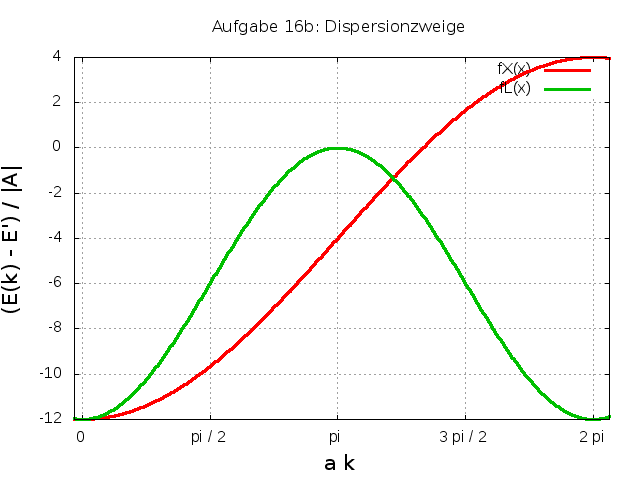
\includegraphics[width=7.5cm]{aufgabe16b.png}
\label{bild16b}
\end{wrapfigure}
Im LCAO-Modell beschreibt das Austauschintegral A den Overlap der Wellenfunktion
eines (Valenz-)Elektrons mit den Wellenfunktionen der (Valenz-)Elektronen benachbarter
Atome. Daraus resultiert eine Aufspaltung der Bänder; diese ist propotional zu A
und einem Geometriefaktor (runde Klammer in obiger Formel) und ist dadurch
auch abhängig von $\vec k$.
\newline
\subsubsection*{b)}
\begin{itemize}
\item[$\Gamma$ X:]
  In $\Gamma$X-Richtung ist $k_y = k_z = 0$, sei $k:= k_x$, dann wird \eqref{eq-disp}
  wegen $\cos(0) = 1$:
\begin{align*}
    E(k) = E'_\alpha - 4\;|A| \left(1 + 2 \cos\frac{k a}{2} \right)
\end{align*}
Siehe rote Kurve fX im Plot. Da $\cos(k)$ Werte zwischen -1 und +1 annehmen kann
ergibt sich eine Bandbreite $B = 16\;|A|$.
\item[$\Gamma$ L:]
  In $\Gamma$L-Richtung ist $k_x = k_y = k_z =: k$, dann wird \eqref{eq-disp}:
\begin{align*}
    E(k) = E'_\alpha - 4\;|A| \left(3 \cos^2\frac{k a}{2} \right)
\end{align*}
Siehe grüne Kurve fL im Plot. Da $\cos^2(k)$ Werte zwischen 0 und +1 annehmen kann
ergibt sich eine Bandbreite $B = 12\;|A|$.
\end{itemize}

\subsubsection*{c)}
Die im Aufgabenblatt rot eingezeichneten Basisvektoren des zweidimensionalen
hexagonalen Gitters haben die Koordinaten
\begin{align*}
  \vec a_1 = a \cdot \begin{pmatrix} 1 \\ 0 \\ 0 \end{pmatrix} \;; \qquad
  \vec a_2 = a \cdot \begin{pmatrix} \cos(120^\circ)\\ \sin(120^\circ)\\ 0\end{pmatrix} =
  a \cdot \begin{pmatrix} -\frac{1}{2}\\\frac{1}{2} \sqrt{3}\\ 0 \end{pmatrix}
\end{align*}
(Zur Berechnung der inversen Gittervektoren ein kurzer Ausflug in drei Dimensionen.)
Damit wird $ | \vec a_1 \times \vec a_2 | = \frac{1}{2} \sqrt{3} a^2$ und für die
Basisvektoren im inversen Gitter ergibt sich:
\begin{align*}
\vec b_1 =  \frac{2 \pi}{\frac{1}{2} \sqrt{3} a^2} (\vec a_2 \times \vec e_3 ) =
  \frac{2 \pi}{a} \begin{pmatrix} 1 \\ 1 / \sqrt{3} \\ 0 \end{pmatrix} \;; \qquad
  \vec b_2 =  \frac{2 \pi}{\frac{1}{2} \sqrt{3} a^2} (\vec e_3 \times \vec a_1) =
  \frac{2 \pi}{a} \begin{pmatrix} 0 \\ 2 / \sqrt{3} \\ 0 \end{pmatrix}
\end{align*}
Man verifiziert leicht: $\vec a_i \cdot \vec b_j = 2 \pi \delta_{ij}$. Jetzt wieder
zweidimensional: Im Real-Raum hat ein Atom im Koordinatenursprung 6 nächste Nachbarn
mit den Koordinaten $R_n\;;\;n = 1, \cdots , 6$ im Gegen-Uhrzeigersinn:
\begin{align*}
\left\lbrace R_n\right\rbrace &= \left\lbrace
 \vec a_1,\; \vec a_1 + \vec a_2,\; \vec a_2, -\vec a_1,\; -\vec a_1 - \vec a_2,\; - \vec a_2
  \right\rbrace
\intertext{Für die Dispersion gilt im LCAO-Modell mit der "`nächste-Nachbarn-Annäherung"':}
\epsilon(\vec k) &= \epsilon'_\alpha - |A| \sum_{n = 1}^6 \mathrm e^{i \vec k \vec R_n}
\intertext{Für das unterste Band ist $\vec k =  \frac{a}{2 \pi}\left(1 \cdot k_x \vec b_1 + 1 \cdot k_y \vec b_2 \right)$, damit wird}
\left\lbrace \vec k \vec R_n \right\rbrace &= \left\lbrace
  a k_x\;, \;a k_x + a k_y\;, \;a k_y\;, \;-a k_x\;, \;-a k_x- a k_y\;, \;-a k_y \right\rbrace \\
\sum_{n = 1}^6 \mathrm e^{i \vec k \vec R_n} &= \\
&= \\
&= 2 \left[ \cos(a k_x) + 2 \cos \left(\frac{a}{2}k_x \right)\cos \left(\frac{\sqrt{3}a}{2}k_y \right) \right]
\end{align*}


% \newpage
\subsection*{Aufgabe 18}
Im folgenden ist zu zeigen, dass die LCAO: $ \phi_{\vec k}(\vec r) := \sum_{\vec R} \mathrm{e}{i\vec k\cdot \vec R}\psi_A(\vec r - \vec R)$ die Eigenschaften einer Bloch Funktion erfüllt.
\subsubsection*{a)}
Zu zeigen ist, dass sich bei einer Verschiebung von $\vec k$ um einen reziproken Gittervektor $\vec G$ die Wellenfunktion nicht ändert:
\begin{align*}
\phi_{(\vec k+\vec G)}(\vec r) \overset{!}{=} \phi_{\vec k}(\vec r)\\
\sum_{\vec R} \mathrm{e}^{i(\vec k+\vec G)\cdot \vec R}\psi_A(\vec r - \vec R) {!}{=} \sum_{\vec R} \mathrm{e}^{i\vec k\cdot \vec R}\psi_A(\vec r - \vec R)\\
\sum_{\vec R} \mathrm{e}^{i\vec G \cdot \vec R}\mathrm{e}^{i\vec k\cdot \vec R}\psi_A(\vec r - \vec R) \overset{!}{=} \sum_{\vec R} \mathrm{e}^{i\vec k\cdot \vec R}\psi_A(\vec r - \vec R)\\
\intertext{Da $\vec G \cdot \vec R = n2\pi$ ist $\mathrm{e}^{i\vec G \cdot \vec R} = 1$ und wir erhalten:}\\
\sum_{\vec R} \mathrm{e}^{i(\vec k\cdot \vec R}\psi_A(\vec r - \vec R) \overset{!}{=} \sum_{\vec R} \mathrm{e}^{i\vec k\cdot \vec R}\psi_A(\vec r - \vec R)\\
\end{align*}
Die letzte Gleichung ist eindeutig erfüllt somit stimmt auch die ursprüngliche Annahme
\subsubsection*{b)}
Zu zeigen ist, dass sich bei der Verschiebung um einen beliebigen Gittervektor $R'$ die Wellenfunktion nicht ändert:
\begin{align*}
\phi_{\vec k}(\vec r+\vec R') \overset{!}{=} \phi_{\vec k}(\vec r)\\
\sum_{\vec R} \mathrm{e}^{i\vec k\cdot \vec R}\psi_A(\vec r + \vec R' - \vec R) \overset{!}{=} \sum_{\vec R} \mathrm{e}^{i\vec k\cdot \vec R}\psi_A(\vec r - \vec R)\\
\sum_{\vec R} \mathrm{e}^{i\vec k\cdot \vec R}\psi_A(\vec r + (\vec R' - \vec R)) \overset{!}{=} \sum_{\vec R} \mathrm{e}^{i\vec k\cdot \vec R}\psi_A(\vec r - \vec R)\\
\intertext{Mit $\vec R'' = \vec R' -\vec R$ wobei $\vec R''$ wieder ein Gittervektor ist:}\\
\sum_{\vec R''} \mathrm{e}^{i\vec k\cdot \vec R}\psi_A(\vec r + \vec R'') \overset{!}{=} \sum_{\vec R} \mathrm{e}^{i\vec k\cdot \vec R}\psi_A(\vec r - \vec R)\\
\end{align*}

Diese Gleichung ist eindeutig erfüllt, da sich die Summen nur in ihrer Bennenung unterscheiden. Anschaulich lässt sich auch sagen: bBei einer Summation über alle Gitterplätze macht es keinen unterschied, wenn man das gesammte Gitter um beliebig viele Gitterplätze in eine Richtung weiterbewegt, der Wert der Summe kann sich dadurch nicht ändern


% \newpage
\subsection*{Aufgabe 19}

\subsubsection*{a)}
\begin{figure}[!ht]
  \centering
  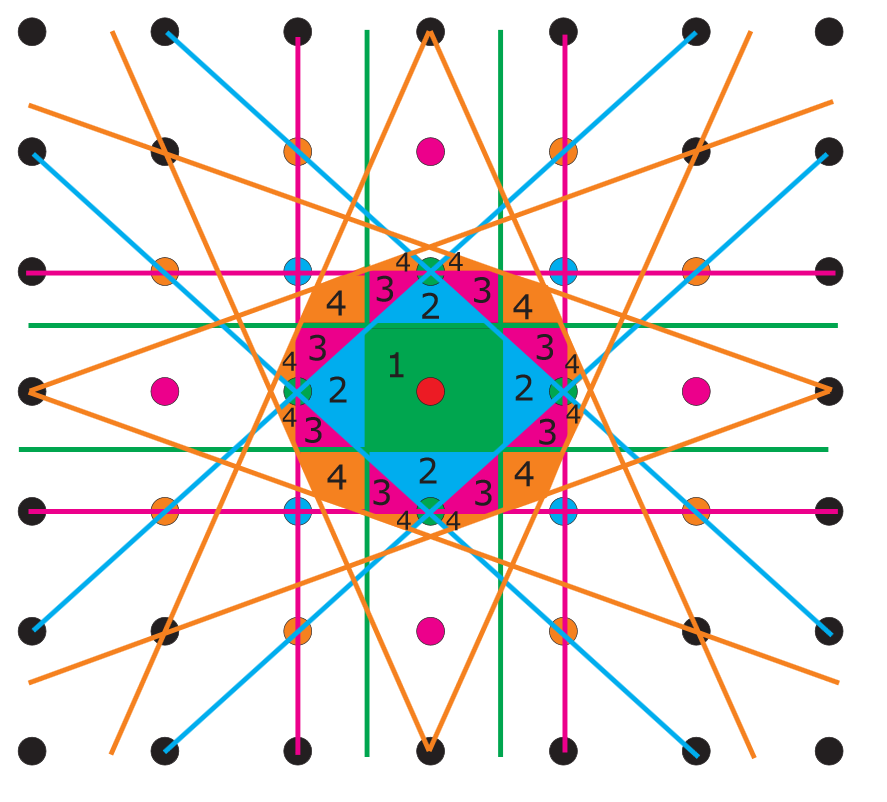
\includegraphics[width=16cm]{aufgabe19a.png}
\end{figure}

\subsubsection*{b)}



\end{document}

